\documentclass[12pt]{report}
\usepackage[margin=1cm, top=1.5cm, bottom=1.5cm]{geometry}
\usepackage{minted}
\usepackage{xcolor}
\usepackage{tcolorbox}
\usepackage{babel}
\usepackage[T1]{fontenc}
\usepackage{textcomp}
\usepackage{titlesec}
\usepackage[hidelinks]{hyperref}
\usepackage{bookmark}
\usepackage{pdfpages}
\usepackage{tikz}
\usetikzlibrary{calc}
\tcbuselibrary{minted}

\renewcommand{\theFancyVerbLine}{\textcolor{gray!50}{\scriptsize\arabic{FancyVerbLine}}}
\renewcommand{\contentsname}{Tartalomjegyzék}

\definecolor{getColor}{HTML}{4CAF50}
\definecolor{postColor}{HTML}{2196F3}
\definecolor{patchColor}{HTML}{FF9800}
\definecolor{deleteColor}{HTML}{F44336}
\definecolor{putColor}{HTML}{9C27B0}

\newcommand{\httpGet}[1]{\colorbox{getColor}{\textbf{\textcolor{white}{GET}}}~#1}
\newcommand{\httpPost}[1]{\colorbox{postColor}{\textbf{\textcolor{white}{POST}}}~#1}
\newcommand{\httpPatch}[1]{\colorbox{patchColor}{\textbf{\textcolor{white}{PATCH}}}~#1}
\newcommand{\httpDelete}[1]{\colorbox{deleteColor}{\textbf{\textcolor{white}{DELETE}}}~#1}
\newcommand{\httpPut}[1]{\colorbox{putColor}{\textbf{\textcolor{white}{PUT}}}~#1}

\titleformat{\chapter}
  {\normalfont\Huge\bfseries}
  {\thechapter.}
  {0.5em}                      
  {} 

\newtcolorbox{codeblock}[2][]{
  colback=black!85!gray,
  colframe=black!50!gray, % Gradient effect
  colbacktitle=black!50!gray,
  coltitle=white,
  title={\ttfamily#2},
  fonttitle=\footnotesize\bfseries,
  arc=5pt,
  boxrule=1pt,
  toptitle=4pt,
  bottomtitle=2pt,
  left=25pt,
  right=5pt,
  top=2pt,
  bottom=2pt,
  % sharp corners=south,
  #1
}

\begin{document}

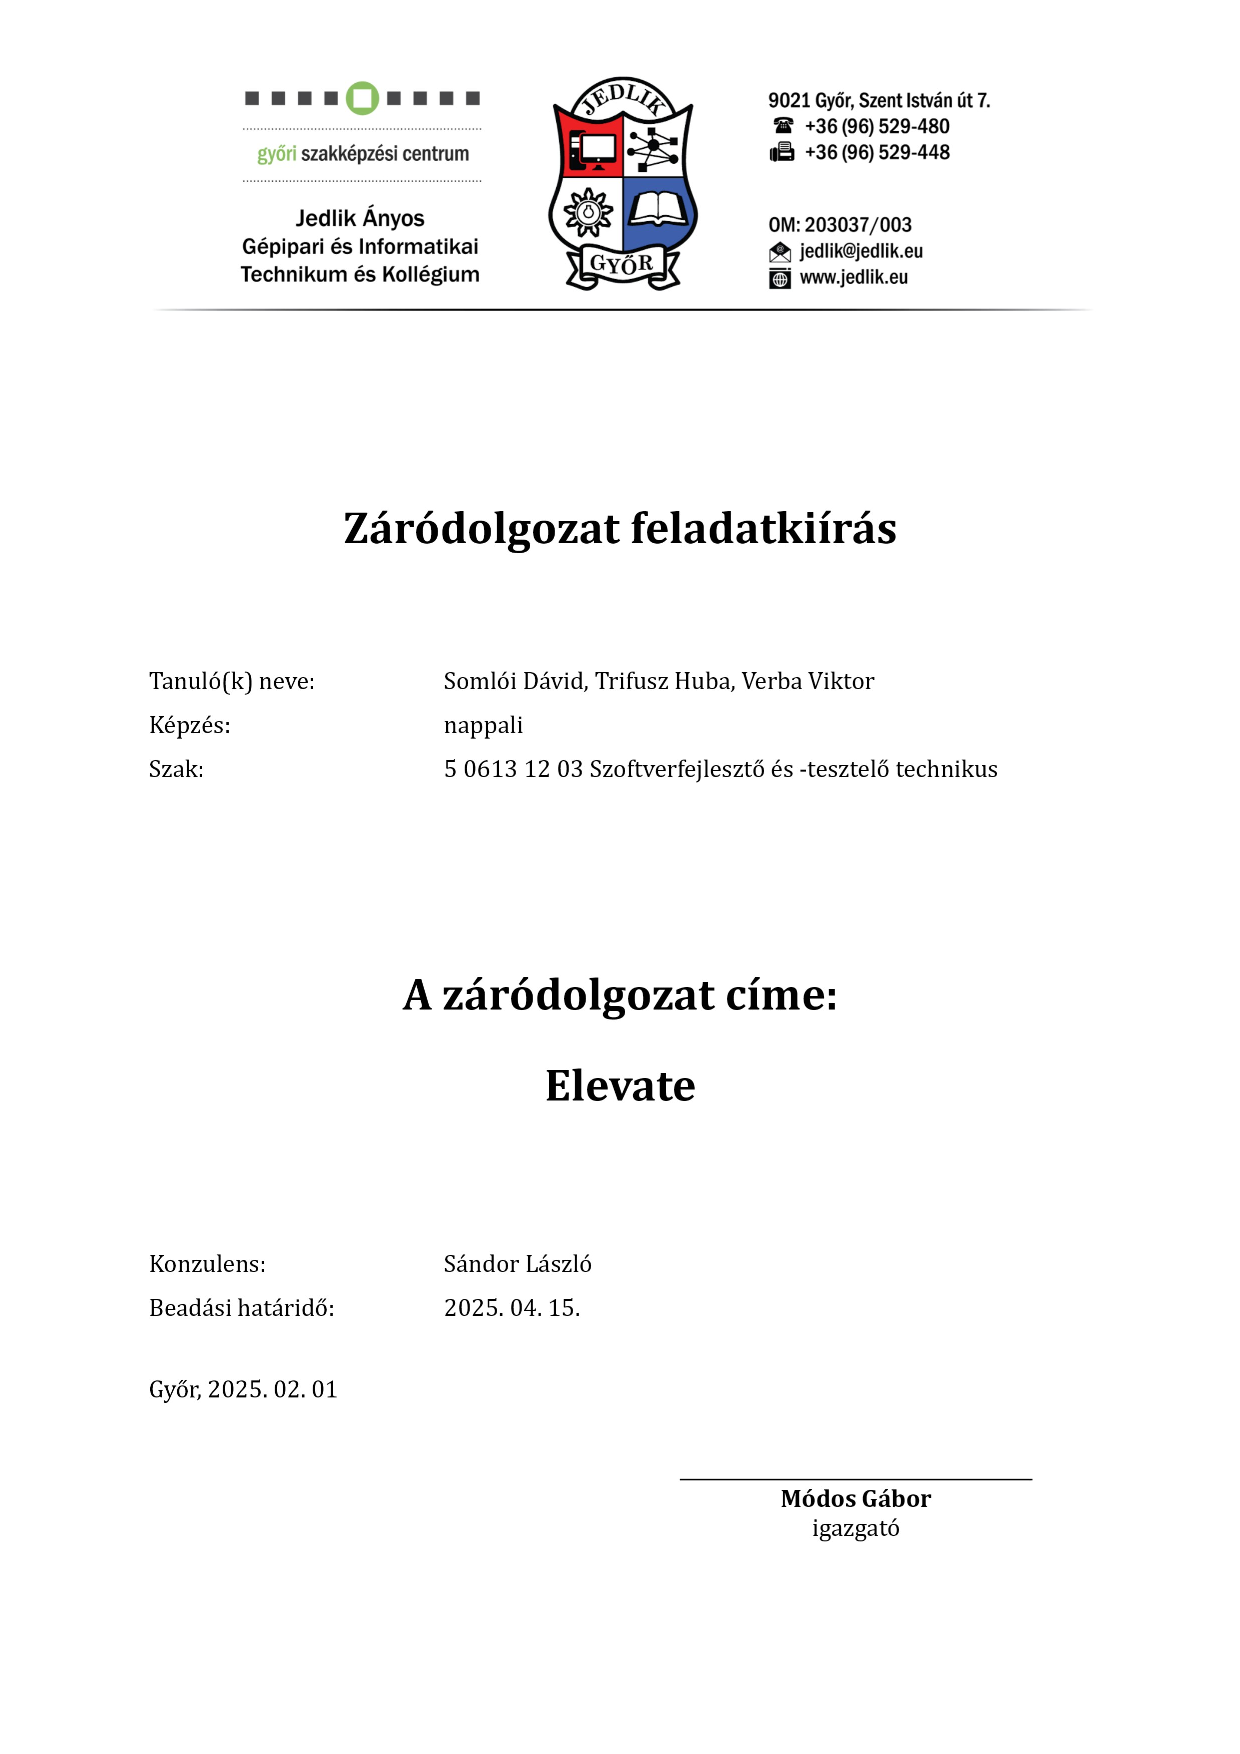
\includepdf[pages=-]{src/cover.pdf}

\setcounter{tocdepth}{3}
\tableofcontents

\chapter{A projektről}
\begin{sloppypar}
A téma kiválasztásánál arra törekedtünk, hogy egy, a hétköznapi élet során alkalmazható szoftvert készítsünk. Több opció is felmerült, azonban végül egy szokásformáló felület mellett döntöttünk, amit Elevate-nek neveztünk el, az egészséges, felemelő életmód jegyében. Az Elevate ösztönzi a felhasználókat, hogy új, pozitív szokásokat vezessenek be, miközben hatékonyan követhetik saját fejlődésüket, emellett hozzájárul életminőségük javításához és a fenntartható fejlődéshez.
\end{sloppypar}
\section{Az Elevate célja}
\begin{sloppypar}
A szoftver célja, hogy a kliens az általa kívánt szokásokat fejlessze, vagy újakat építsen be a napirendjébe. Például, ha a felhasználó a dohányzásról szeretne leszokni, akkor monitorozni tudja a fogyasztását és különféle jutal-makat kap, ha tartja a felállított célját. Nem csak a rossz szokások követését biztosítja az applikáció, pozitív célokat is ki lehet tűzni, mint “Napi 10 fekvőtámasz" vagy “Hetente kitakarítani”. Egy szokás tartásához elengedhet-etlen, hogy a beállított gyakorisággal teljesítsük a kitűzött kihívásokat. Ennek megkönnyítése érdekében az Elevate egy naptárszerű nézetben jeleníti meg a teendőket és emlékeztet azok elvégzésére. 
\end{sloppypar}
\chapter{Weboldal}
\chapter{Mobil Applikáció}
\chapter{Adatbázis}
\section{Adatbázis tervezés}
Az Elevate két különböző adatbázis rendszert támogat a különböző környezetekben való futtatáshoz:
\begin{itemize}
  \item Fejlesztési környezetben: MySQL
  \item Production környezetben: PostgreSQL
\end{itemize}

Erre azért van így, mert a fejlesztést MySQL-el kezdtük, majd a Koyeb-re való publikáláshoz szükségessé vált PostgreSQL kompatibilitás. Az adatbázis migrációk kezelésére az Entity Framework Core migrációs rendszerét használjuk, amely lehetővé teszi a séma verziókövetését és az adatbázis automatikus frissítését, ez kisebb módosításokkal mindkét adatbázis környezettel megfelelően működik.

\section{Entitások és kapcsolatok}
Az adatbázis séma a következő fő táblákat tartalmazza:

\begin{figure}[H]
    \centering
    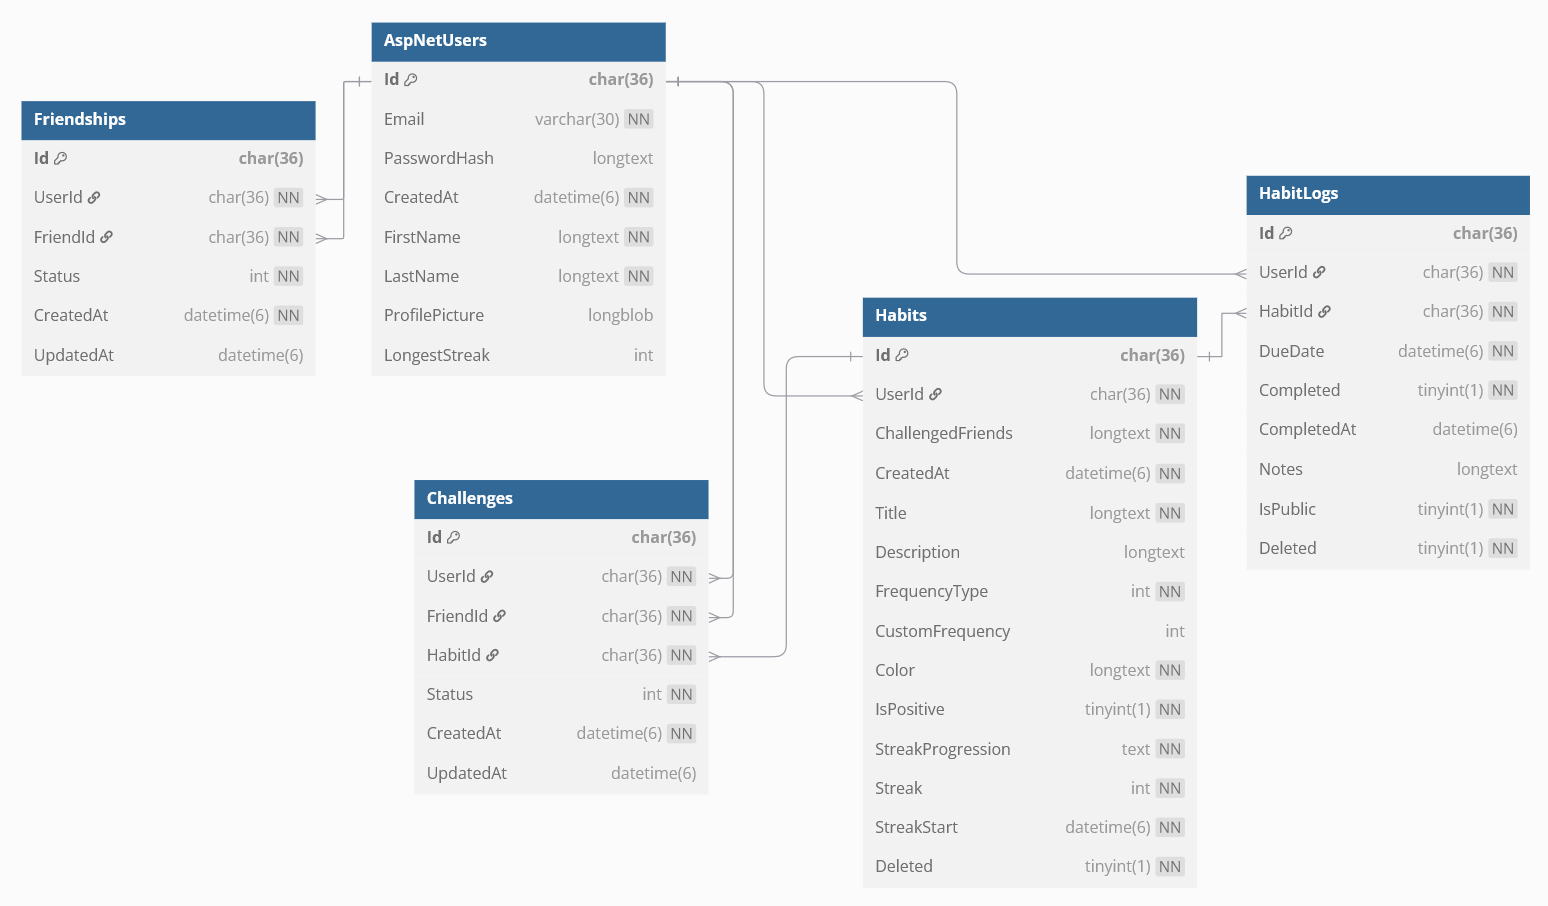
\includegraphics[width=0.9\textwidth]{src/dbdiagram.png}
    \label{fig:database-diagram}
\end{figure}

\section{Adatbázis biztonsági megfontolások}
\begin{itemize}
  \item A jelszavak hash-elve tárolódnak az adatbázisban (ASP.NET Core Identity)
  \item Adatbázis migrációk verziókövető rendszerben tárolva
  \item A kapcsolatok integritása constraint-ekkel biztosítva
  \item Indexek használata a gyakori lekérdezések optimalizálására
\end{itemize}

\section{Adatbázis elérés}
Az adatbázis elérését a DbConnectionManager osztály biztosítja az alábbi módon:
\begin{codeblock}{DbConnectionManager.cs}
  \inputminted[
    style=one-dark,
    breaklines,
    linenos,
    firstline=24,
    lastline=38,
    gobble=8
    ]{csharp}{/home/smapesz/code/elevate/Backend/Elevate.Data/Database/DbConnectionManager.cs}
\end{codeblock}

Majd az így kapott kapcsolattal a DbContext osztály alkot egy, a későbbiekben feldolgozható adatszerkezetet.
\begin{codeblock}{ElevateDbContext.cs}
  \inputminted[
    style=one-dark,
    breaklines,
    linenos,
    firstline=61,
    lastline=72,
    gobble=8
    ]{csharp}{/home/smapesz/code/elevate/Backend/Elevate.Data/Database/ElevateDbContext.cs}
\end{codeblock} 

\chapter{Backend}

\section{Technológia}
Az Elevate backend rendszere ASP.NET Core alapú, Entity Framework Core ORM-mel. Az adatbázis és a backend kapcsolata model first elv alapján lett létrehozva. Az API RESTful elvek alapján lett kialakítva és a CRUD (Create, Read, Update, Delete) műveleteket valósítja meg.

\section{Architektúra}
A backend a következő komponensekből épül fel:
\begin{itemize}
  \item \textbf{Modellek} - Az adatmodelleket és adatbázis entitásokat reprezentálják
  \item \textbf{DTO-k (Data Transfer Objects)} - Adatok átvitelére szolgáló objektumok a rétegek között, illetve a kliens és szerver között
  \item \textbf{Repository-k} - Az adatbázissal való kommunikációért felelősek, CRUD műveletek végrehajtása
  \item \textbf{Kontrollerek} - A kérések feldolgozása, autentikáció és authorizáció kezelése, valamint a válaszok generálása
  \item \textbf{Service-k} - Az üzleti logika megvalósítása
  \item \textbf{Middleware} - Kivételek kezelése és egyéb előfeldolgozási feladatok
  \item \textbf{Segédosztályok} - Általános funkciók és segédszolgáltatások
\end{itemize}

\section{Végpontok}
A Backend API részletes dokumentációja a \href{https://elevate.koyeb.app/swagger}{\textcolor{blue}{\underline{Swagger}}} felületen érhető el. Az alábbiakban a főbb végpontok láthatóak:

\begin{itemize}
  \item \textbf{Autentikáció}
    \begin{itemize}
      \item Regisztráció (\httpPost{/api/auth/register})
      \item Bejelentkezés (\httpPost{/api/auth/login})
    \end{itemize}
  \item \textbf{Felhasználó}
    \begin{itemize}
      \item Felhasználó adatainak lekérése email alapján (\httpGet{/api/user})
      \item Felhasználó adatainak lekérése id alapján (\httpGet{/api/user/:id})
      \item Felhasználó adatainak frissítése (\httpPatch{/api/user/:id})
    \end{itemize}
  \item \textbf{Szokások}
    \begin{itemize}
      \item Szokások listázása (\httpGet{/api/habit})

      \item Szokás lekérése azonosító alapján (\httpGet{/api/habit/:id})
      \item Új szokás létrehozása (\httpPost{/api/habit})
      \item Szokás módosítása (\httpPatch{/api/habit/:id})
      \item Szokás törlése (\httpDelete{/api/habit/:id})
    \end{itemize}
  \item \textbf{Szokás napló}
    \begin{itemize}
      \item Szokás naplók listázása (\httpGet{/api/habitlog})
      \item Szokás napló lekérése azonosító alapján (\httpGet{/api/habitlog/:id})
      \item Napi szokás naplók lekérése (\httpGet{/api/habitlog/:dueDate})
      \item Szokás napló frissítése (\httpPatch{/api/habitlog/:id})
    \end{itemize}
  \item \textbf{Kihívások}
    \begin{itemize}
      \item Kihívások lekérése felhasználó azonosító alapján (\httpGet{/api/challenge/:userId/challenges})
      \item Kihívás meghívók listázása (\httpGet{/api/challenge/:userId/challenge-invites})
      \item Elküldött kihívás meghívók listázása (\httpGet{/api/challenge/:userId/sent-challenge-invites})
      \item Új kihívás létrehozása (\httpPost{/api/challenge})
      \item Kihívás státuszának frissítése (\httpPatch{/api/challenge})
      \item Kihívás törlése (\httpDelete{/api/challenge})
    \end{itemize}
  \item \textbf{Feed}
    \begin{itemize}
      \item Feed bejegyzések lekérése (\httpGet{/api/feed})        
    \end{itemize}
  \item \textbf{Barátok}
    \begin{itemize}
      \item Barátok listázása (\httpGet{/api/friendship/:userId/friends})
      \item Beérkezett barátkérések lekérése (\httpGet{/api/friendship/:userId/fried-requests})
      \item Küldött barátkérések lekérése (\httpGet{/api/friendship/:userId/friend-requests-sent})
      \item Barátkérés küldése (\httpPost{/api/friendship})
      \item Barátkérés elfogadása/elutasítása (\httpPatch{/api/friendship})
      \item Barátság törlése (\httpDelete{/api/friendship})
    \end{itemize}
\end{itemize}

\section{Autentikáció és biztonság}
Az API biztonságos használatához JWT (JSON Web Token) alapú autentikáció van implementálva. A működése:
\begin{itemize}
  \item A felhasználó bejelentkezéskor egy JWT tokent kap(aszimmetrikus titkosítással)
  \item A token érvényességi ideje korlátozott
  \item A védett végpontok eléréséhez a tokent minden kérés fejlécében el kell küldeni
\end{itemize}

A biztonság további rétegei:
\begin{itemize}
  \item Input validáció
  \item CORS védelem (A mobil alkalmazás miatt enyhített)
  \item Jelszó titkosítás
\end{itemize}

\chapter{Tesztelés}

\end{document}